\documentclass[mathserif,serif]{beamer}
\usepackage[utf8]{inputenc}
\usepackage[T1]{fontenc}
\usepackage{graphicx}

\title[Crisis] % (optional, only for long titles)
{Use of Recommender System in Robotics}
\subtitle{R\&D Project Proposal }
\author[Nair, Deebul] % (optional, for multiple authors)
{Deebul Nair}
\institute[Universities Here and There] % (optional)
{
    Advised by:\\
    \textbf{Prof. Dr. Paul Pl{\"o}ger}\\
    \textbf{Iman Awaad}
}
\date[KPT 2004] % (optional)
{\today}
\subject{Computer Science}


%Global Background must be put in preamble\usebackgroundtemplate%
%\includegraphics[width=\paperwidth,height=\paperheight]{newton.jpg}%





\usepackage{amsmath}
\begin{document}
 \frame{\titlepage}
\begin{frame}{Robot Programming by Demonstration (PbD)}
\begin{figure}[htp]
\centering
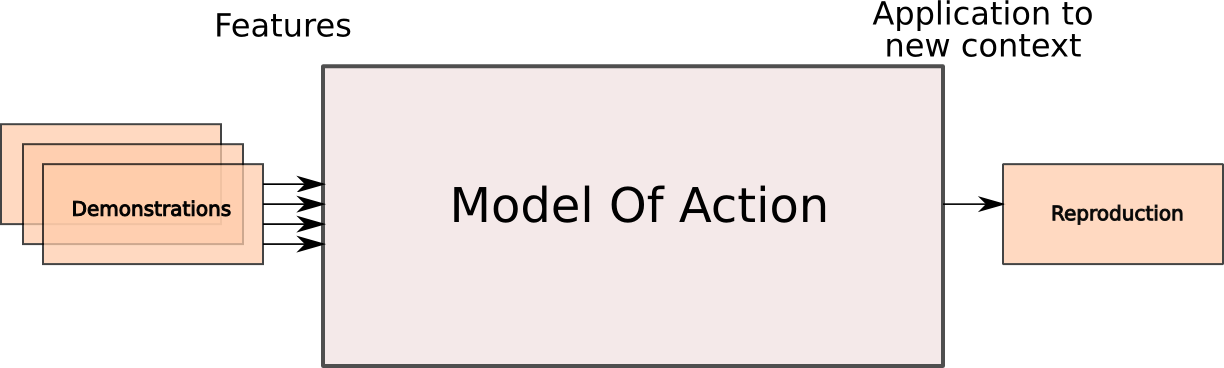
\includegraphics[scale=0.33]{/data/dataDeebul/rnd/RecommenderSystemInRobotics/art/PbD.png}
\caption{Scehmatic of learning process
\footnote{\tiny{A Billard, S Calinon, R Dillmann, S Schaal, Survey: Robot programming by demonstration, MIT Press, 2008, Pg 5}}}
\label{Programming by Demonstration}

\end{figure}
\end{frame}


% Local background must be enclosed by curly braces for grouping.
%{\usebackgroundtemplate{\includegraphics[width=\paperwidth]{kitten.jpg}}%
{\begin{frame}{Modelling the Action: }
\begin{figure}[htp]
\centering
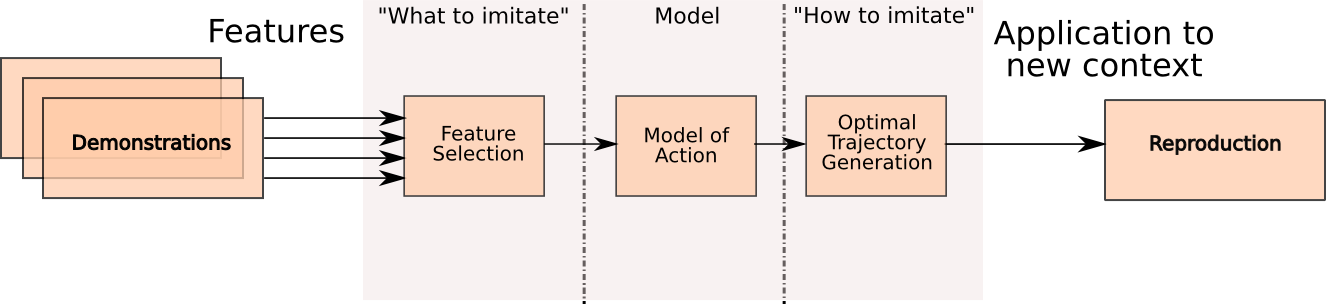
\includegraphics[scale=0.3]{/data/dataDeebul/rnd/RecommenderSystemInRobotics/art/PbD-InDepth.png}
\caption{Components of Modelling the action
\footnote{\tiny{A Billard, S Calinon, R Dillmann, S Schaal, Survey: Robot programming by demonstration, MIT Press, 2008}}}

\label{}
\end{figure}
\end{frame}
}


\begin{frame}{Scope of the R\&D}
\framesubtitle{Inferring what to imitate}
\begin{figure}[htp]
\centering
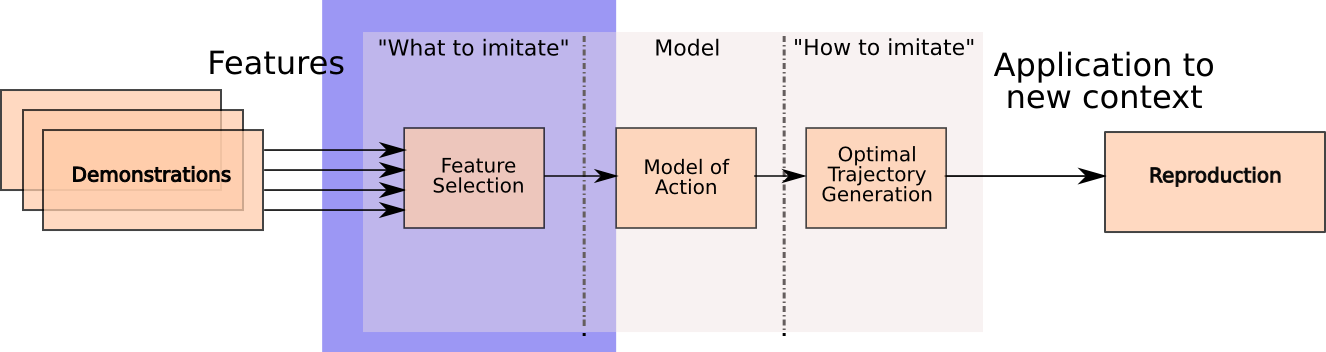
\includegraphics[scale=0.31]{/data/dataDeebul/rnd/RecommenderSystemInRobotics/art/myRnD.png}
\caption{Scope of the R\&D}
\label{}
\end{figure}
\end{frame}
\begin{frame}{Feature Selection: Current Approaches}
\begin{itemize}
	\item Hidden Markov Model [5]
	\item Graph Based [6]
	\item Gaussian Mixture Model [7]
	\item Locally Weighted Regression [8]
	\item Receptive Field Weighted Regression [9]
	\item Locally Weighted Projection Regression[10] 
\end{itemize}
\end{frame}

\begin{frame}{Limitation of Current Approaches}
\setbeamercolor{postit}{fg=black,bg=yellow}
\begin{beamercolorbox}[sep=1em]{postit}
	Large amount of training data required.
\end{beamercolorbox}
\end{frame}
\begin{frame}{Approach}
    \begin{itemize}
	\item Create a set of experts, which determine the relevance of a feature with respect to the action.
	\item Experts\footnote{\tiny{Abdo, N., Spinello, L., Burgard, W., \& Stachniss, C. (n.d.). Inferring What to Imitate in Manipulation Actions by Using a Recommender System. In ICRA (Vol. 31, pp. 189–206) }} : The experts are created by borrowing ideas from the Recommender Systems theory.
	    \item The experts knowledge of manipulation are collected before training.
	    \item Training Demonstrations + Experts = Recommendation of relevant features.
\end{itemize}
\end{frame}
\begin{frame}{Recommender Systems }
    \begin{itemize}
	\item Recommender Systems are software tools and techniques providing suggestions for items to be of use to a user. \footnote{\tiny{Ricci, Francesco, Lior Rokach, and Bracha Shapira. Introduction to recommender systems handbook. Springer US, 2011.}}
	\item Recommender Systems in Movie Recommendation\\
	{\centering
	\begin{tabular}{|l|l|l|}
    \hline
	    Movies & Users & Genre\\
    \hline
	    .. & .. & ..\\
    \hline
    \end{tabular}\\}
    
    \item Recommender Systems in Feature Selection\\
	{\centering
	\begin{tabular}{|l|l|l|}
    \hline
	    Features & Demonstration & Expert\\
    \hline
	    .. & .. & ..\\
    \hline
    \end{tabular}\\}

\end{itemize}
\end{frame}
 \begin{frame}{Summary}
    \begin{itemize}
	\item Formulate a feature selection problem.
	\item Multiple experts will provide recommendation about which  set of features is relevant for an action 
	\item Identify the relevant features with minimum number of demonstrations.
	\item Use case investigation of recommender systems in other fields of robotics.
	
\end{itemize}
\begin{figure}[htp]
\centering
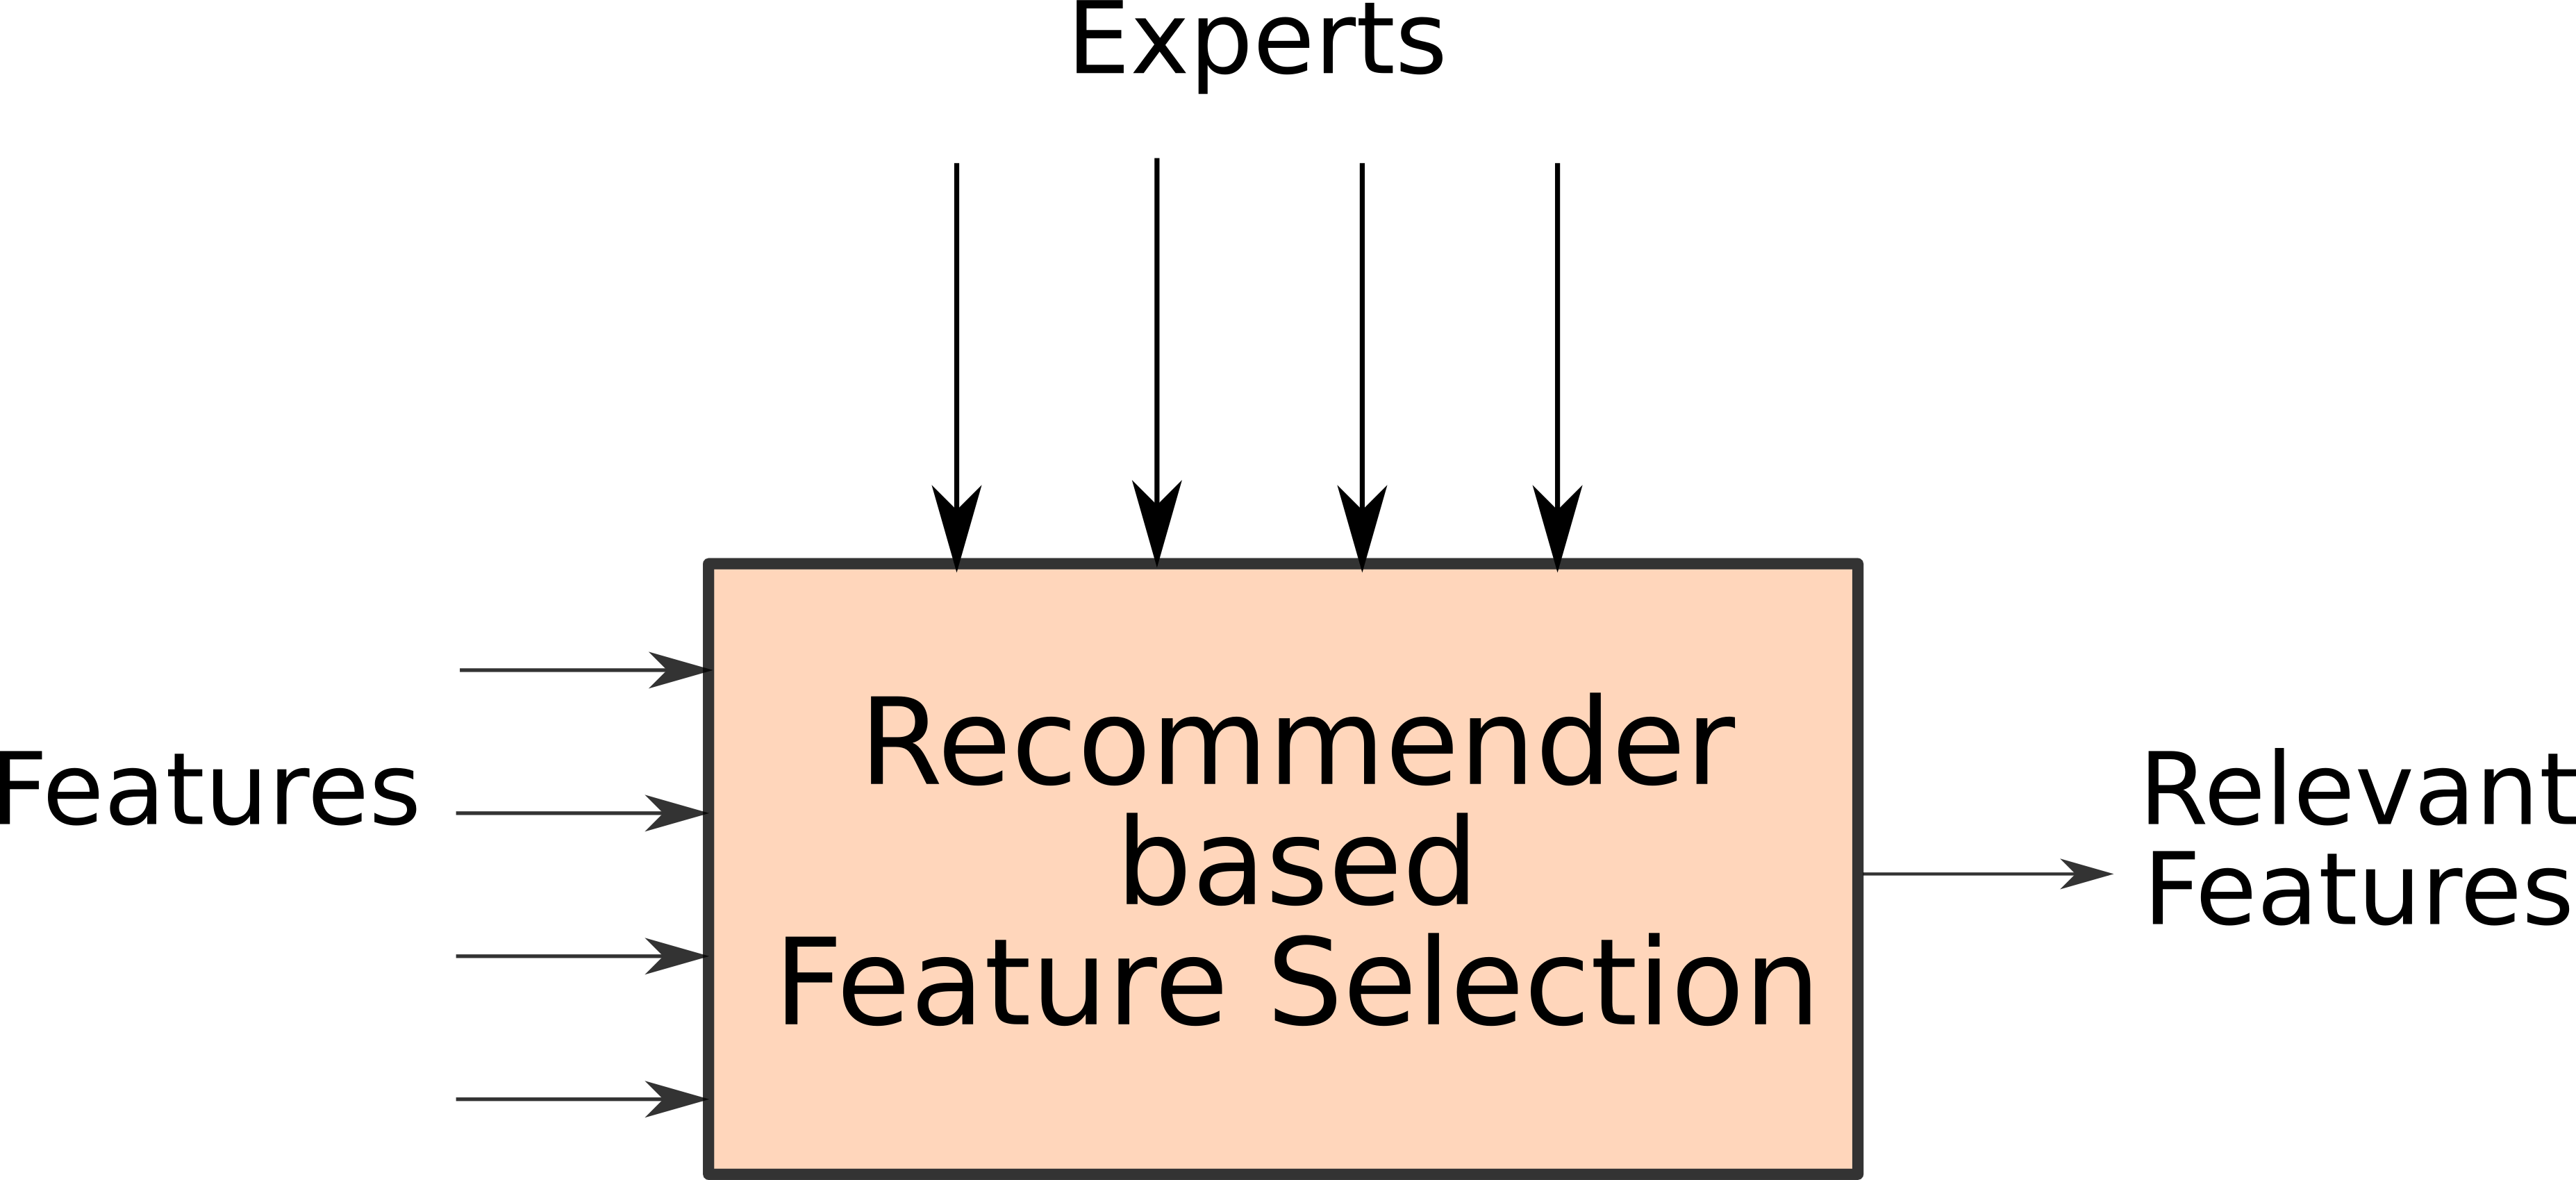
\includegraphics[scale=0.22]{/data/dataDeebul/rnd/RecommenderSystemInRobotics/art/featureSelection.png}
\caption{Recommender based Feature Selection}
\label{}
\end{figure}
\end{frame}
\bibliography{/data/dataDeebul/rnd/RecommenderSystemInRobotics/proposal/RecommenderSystemInRobotics.bib}{}
\bibliographystyle{plain}
\begin{frame}{References:}
\begin{description}
	\item[5] \tiny{T. Inamura, H. Tanie, and Y. Nakamura.
Keyframe compression and decompression for time
series data based on continuous hidden Markov
models. In Proceedings of the IEEE/RSJ international Conference on Intelligent Robots and Systems (IROS), volume 2, pages 1487–1492, 2003.}

	\item[6] M.N. Nicolescu and M.J. Mataric. Natural methods for robot task learning: Instructive demonstrations, generalization and practice. In Proceedings of the International Joint Conference on Autonomous Agents and Multiagent Systems (AAMAS), pages 241–248, 2003.

	\item[7] S. Calinon, F. Guenter, and A. Billard. On learning, representing and generalizing a task in a humanoid robot. IEEE Transactions on Systems,
Man and Cybernetics, Part B. Special issue on
robot learning by observation, demonstration and
imitation, 37(2):286–298, 2007.

	\item[8]  C.G. Atkeson, A.W. Moore, and S. Schaal. Locally
weighted learning for control. Artificial Intelligence
Review, 11(1-5):75–113, 1997.

	\item[9]  S. Schaal and C.G. Atkeson. Constructive incremental learning from only local information. Neural Computation, 10(8):2047–2084, 1998.

	\item[10] S. Vijayakumar, A. D’souza, and S. Schaal. Incremental online learning in high dimensions. Neural
Computation, 17(12):2602–2634, 2005.

\end{description}
\end{frame}
\end{document}